\documentclass[a4paper,10pt]{article}
\usepackage{graphicx}
\usepackage{amsmath}
\usepackage{amssymb}
\usepackage[italian]{babel}
\usepackage[T1]{fontenc}
\usepackage[utf8]{inputenc}
\usepackage[margin=1.25in]{geometry}

\usepackage[backend=biber]{biblatex}
\addbibresource{ref.bib}

\begin{document}

   \title{{\large Universita' degli Studi di Padova \\ } {\normalsize Corso di laurea triennale in Ingegneria Informatica}\\ \vspace{1.8cm} \textbf{ Homework 2: Strumenti per la valutazione delle prestazioni di rete}}
   
   \author{Giacomo Camposampiero, matricola 1187180} 
   \date{20 novembre 2020}
   \maketitle
   \vspace{9.2cm}
   \renewcommand{\contentsname}{Indice}      
   \tableofcontents
   \newpage

\section{Comando \texttt{ping} }
\texttt{ping} (Packet INternet Groper) è un software di amministrazione per reti di computer utilizzato per verificare la raggiungibilità di un host all'interno di una rete IP. Questa applicazione è supportata nella maggior parte dei sistemi operativi comuni ed è ampiamente utilizzata come strumento elementare di diagnostica di rete. \\\\
Il funzionamento di \texttt{ping} è interamente basato sul protocollo ICMP (Internet Control Message Protocol, RFC 792), che si appoggia direttamente ai servizi offerti dall'Internet Protocol, senza coinvolgere alcun tipo di servizio di livello di trasporto. L'applicazione invia una serie di pacchetti ICMP Echo Request ad una destinazione, la quale risponde ad ogni pacchetto ricevuto inviando un corrispettivo pacchetto ICMP Echo Reply di risposta della stessa dimensione della richiesta. Una rappresentazione grafica della struttura di un pacchetto ICMP è riportata in Figura \ref{fig:ICMP}. \texttt{ping} misura il cosiddetto \textit{Round-Trip Time} (RTT), ovvero il tempo che intercorre tra l'invio della richiesta e la ricezione della risposta, per poi visualizzarlo in output.

\begin{figure}[h!]
	\centering
	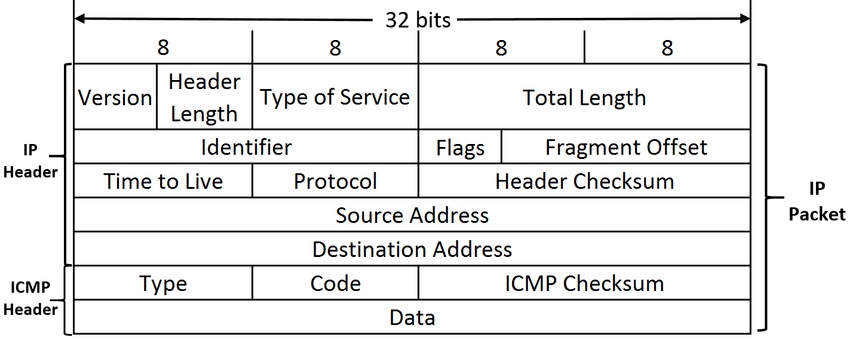
\includegraphics[scale=0.25]{img/icmp.png}
  	\caption{Struttura pacchetto ICMP \cite{ref:icmp}}
  	\label{fig:ICMP}
\end{figure}

\subsection{Opzioni da linea di comando}
Il software \texttt{ping} offre numerose opzioni da linea di comando, che possono variare a seconda del sistema operativo in cui è implementato e dei privilegi posseduti dall'utente che lo invoca. Una lista delle opzioni disponibili può essere ottenuta dall'utente mediante l'invocazione del comando \texttt{man ping}. Di seguito è riportato un elenco delle opzioni che sono state giudicate più utili nella valutazione delle prestazioni di una connessione.
\begin{itemize}

\item \textbf{\texttt{-f}}: Flood ping. For every ECHO REQUEST sent a period “.” is printed, while for ever ECHO REPLY received a backspace is printed. This provides a rapid display of how many packets are being dropped. If interval is not given, it sets interval to zero and outputs packets as fast as they come back or one hundred times per second, whichever is more. Only the super-user may use this option with zero interval.

\item \textbf{\texttt{-i interval}}: Wait interval seconds between sending each packet. The default is to wait for one second between each packet normally, or not to wait in flood mode. Only super-user may set interval to values less than 0.2 seconds.

\item \textbf{\texttt{-m mark}}: use mark to tag the packets going out. This is useful for variety of reasons within the kernel such as using policy routing to select specific outbound processing.

\item \textbf{\texttt{-O}}: Report outstanding ICMP ECHO reply before sending next packet. This is useful together with the timestamp -D to log output to a diagnostic file and search for missing answers.

\item \textbf{\texttt{-p pattern}}: You may specify up to 16 “pad” bytes to fill out the packet you send. This is useful for diagnosing data-dependent problems in a network. For example, -p ff will cause the sent packet to be filled with all ones.

\item \textbf{\texttt{-Q tos}}: Set Quality of Service -related bits in ICMP datagrams.  tos can be decimal (ping only) or hex number.

\item \textbf{\texttt{-R}}: ping only. Record route. Includes the RECORD ROUTE option in the ECHO REQUEST packet and displays the route buffer on returned packets. Note that the IP header is only large enough for nine such routes. Many hosts ignore or discard this option.

\item \textbf{\texttt{-T timestamp option}}: Set special IP timestamp options.  timestamp option may be either tsonly (only timestamps), tsandaddr (timestamps and addresses) or tsprespec host1 [host2 [host3 [host4]]] (timestamp prespecified hops).

\item \textbf{\texttt{-U}}:  Print full user-to-user latency (the old behaviour). Normally ping prints network round trip time, which can be different f.e. due to DNS failures.

\item \textbf{\texttt{-w deadline}}: Specify a timeout, in seconds, before ping exits regardless of how many packets have been sent or received. In this case ping does not stop after count packet are sent, it waits either for deadline expire or until count probes are answered or for some error notification from network.

\item \textbf{\texttt{-W timeout}}: Time to wait for a response, in seconds. The option affects only timeout in absence of any responses, otherwise ping waits for two RTTs.
\end{itemize}
Per quanto riguarda invece le opzioni che permettono l'attivazione di specifiche funzionalità definite nella consegna, ne è stata verificata l'esistenza e riportato il formato di seguito.
\begin{itemize}

\item \textbf{\texttt{-c count}}: dopo aver inviato \textit{count} pacchetti ECHO REQUEST, ne interrompe l'invio, rimanendo in attesa dei \textit{count} pacchetti ECHO REPLY (se utilizzato insieme ad opzioni che permettono di specificare una deadline, \texttt{ping} aspetta al massimo fino a che il timeout non termina e alcune request potrebbero non ricevere risposta) 

\item \textbf{\texttt{-s packetsize}}: specifica il numero di data byte da inviare. Il default corrisponde a 56 data bytes, che si traducono in una dimensione totale del pacchetto di 64 ICMP data bytes considerando anche gli 8 bytes dell'header. Si ricorda inoltre che la dimensione dei pacchetti IP è in ogni caso maggiore rispetto a questa, in quanto vengono aggiunti 20 bytes di header IP.

\item \textbf{\texttt{-t ttl}}: permette di definire il campo \textit{Time-To-Live} (TTL) dell'header IP. 

\end{itemize}

\newpage
\subsection{Time-To-Live e Round-Trip Time}
Il \textit{Time-To-Live} (TTL) è una campo dell'header IP che viene impostato dal mittente e decrementato ogni volta che il pacchetto è inoltrato da un nodo intermedio nella rete. Se un nodo che non è il destinatario finale riceve un pacchetto il cui TTL è pari ad 1, il campo è decrementato ed il pacchetto scartato. Pertanto, il TTL determina il numero di inoltri (hop) che un pacchetto può subire prima di raggiungere la destinazione.\\\\
Al fine di testare il numero di hop che separano la macchina da cui sono stati svolti gli esperimenti dal server destinazione (88.80.187.84) è stato scritto un breve script di shell Linux, riportato di seguito.
\begin{quote}
\begin{verbatim}
echo "Time-To-Live Experiment" > ttl.txt
for i in  8 9 10 11 12 13 14 15 
do
  echo "TTL $i" >> ttl.txt
  ping -q -c 15 -t $i 88.80.187.84 >> ttl.txt
done
\end{verbatim}
\end{quote}
Questo script permette di testare il comando \texttt{ping} specificando diversi valori di TTL ($\in[8, 15]$) e di salvare i risultati ottenuti in un file denominato \texttt{ttl.txt}. In questo modo risulta possibile verificare per che valore di soglia i pacchetti smettono di essere scartati da nodi intermedi e arrivano effettivamente al server destinazione. Il valore di hop tra la macchina mittente e il server di destinazione è stato sperimentalmente verificato essere \textbf{$13$}.\\\\
Il \textit{Round-Trip Time} (RTT) corrisponde invece alla somma dei ritardi accumulati nel percorso di andata (tra sorgente e destinazione) e di ritorno (viceversa). Numerando da 1 a \textit{n} i nodi attraversati durante l'intero tragitto comprensivo di andata e ritorno, il RTT del \textit{k}-esimo scambio request-reply può essere calcolato come
\begin{align*}
RTT(k) = \sum_{i=1}^{n} \left( \frac{L(k)}{R_i} + q_i(k) + \tau_i \right)
\end{align*}
dove
\begin{itemize}
\item $L(k)$ è la dimensione a livello rete (IP) della PDU che trasporta i pacchetti Request/Reply delkesimo ciclo.  Detta $l(k)$ la lunghezza del payload del pacchetto ICMP Echo Request/Reply, e considerando che il protocollo ICMP aggiunge 8 byte di header, e il protocollo IP altri 20 byte di header, si haL(k) =`(k) + 28×8[bit] a livello IP.
\item $R_i$ è il bitrate offerto dal link \textit{i}-esimo a livello rete (ovvero, il throughput visto del protocollo di rete IP) in bit/s.
\item $q_i(k)$ è il tempo speso dal pacchetto nel buffer di trasmissione del link \textit{i}-esimo.
\item $\tau_i$ è il tempo di propagazione lungo il link \textit{i}-esimo.
\end{itemize}

\newpage

\section{References}
\printbibliography[heading=none]

\end{document}